\documentclass{tikzposter} %Options for format can be included here

\usepackage{todonotes}

\usepackage[tikz]{bclogo}
\usepackage{lipsum}
\usepackage{amsmath}

\usepackage{booktabs}
\usepackage{longtable}
\usepackage[absolute]{textpos}
\usepackage[it]{subfigure}
\usepackage{graphicx}
\usepackage{cmbright}
%\usepackage[default]{cantarell}
%\usepackage{avant}
%\usepackage[math]{iwona}
\usepackage[math]{kurier}
\usepackage[T1]{fontenc}


%% add your packages here
\usepackage{hyperref}
% for random text
\usepackage{lipsum}
\usepackage[english]{babel}
\usepackage[pangram]{blindtext}

\colorlet{backgroundcolor}{blue!10}

% Title, Author, Institute
\title{Ordinal Regression with a Tabular Wine Quality Dataset}
\author{Sen Han$^1$, Gang Li$^2$}
\institute{$^1$ Beijing Technology and Business University, China \\
	$^2$ Deakin University, Australia
}
%\titlegraphic{logos/tulip-logo.eps}

%Choose Layout
\usetheme{Wave}


\begin{document}
	
	
	\colorlet{blocktitlebgcolor}{blue!23}
	
	% Title block with title, author, logo, etc.
	\maketitle
	
	\begin{columns}
		% FIRST column
		\column{0.5}% Width set relative to text width
		
		%%%%%%%%%% -------------------------------------------------------------------- %%%%%%%%%%
		\block{Introduction}{
			
			Ordinal regression was conducted on a dataset derived from a deep learning model trained on the quality dataset of red variants of the "Vinho Verde" wine from Spain. This dataset characterizes the impact of various chemical substances present in wine on its quality. The quality grades are ordinal and imbalanced, with common wines being significantly more prevalent than either high-quality or low-quality wines.
			
		}
		%%%%%%%%%% -------------------------------------------------------------------- %%%%%%%%%%
		
		
		%%%%%%%%%% -------------------------------------------------------------------- %%%%%%%%%%
		\block{Preliminaries}{
			
			Smote
			
			In the provided dataset, the samples with quality grades 5 and 6 are substantially more numerous than those of other grades, necessitating a consideration of the potential impacts of employing the SMOTE technique.
			SMOTE (Synthetic Minority Over-sampling Technique) is a method employed in data science and machine learning to address the issue of class imbalance in classification problems. Class imbalance refers to the scenario where the instance count of one class (the minority class) is significantly lower than that of other classes (the majority classes). This imbalance can lead to biased performance or suboptimal results in machine learning models, as they are often dominated by the majority class and tend to overlook the minority class. 
			By generating synthetic samples, SMOTE aids in reducing the overfitting issues that simple over-sampling might cause.
			
			Kappa
			
			The quadratic weighted kappa is calculated as follows. First, an N x N histogram matrix O is constructed, such that Oi,j corresponds to the number of Ids i (actual) that received a predicted value j. An N-by-N matrix of weights, w, is calculated based on the difference between actual and predicted values:
			
			\[ w_{i,j} = \frac{(i - j)^2}{(N - 1)^2} \]
			
			An N-by-N histogram matrix of expected outcomes, E, is calculated assuming that there is no correlation between values.  This is calculated as the outer product between the actual histogram vector of outcomes and the predicted histogram vector, normalized such that E and O have the same sum.
			
			From these three matrices, the quadratic weighted kappa is calculated as: 
			
			\[ \kappa = 1 - \frac{\sum_{i,j} w_{i,j} O_{i,j}}{\sum_{i,j} w_{i,j} E_{i,j}} \]
			
		}
		%%%%%%%%%% -------------------------------------------------------------------- %%%%%%%%%%
		
		
		%%%%%%%%%% -------------------------------------------------------------------- %%%%%%%%%%
		
		
		\block{Experiment and analysis}{
			To gain an initial understanding of the given dataset, it is imperative to analyze it from multiple perspectives. The first step involves a comprehensive analysis of the dataset itself.
			
			The datasets do not contain any missing values, thus negating the necessity for missing value processing.
			
			An analysis of the target variable and univariate analysis were conducted on both the original and training datasets. The following figure illustrates the composition of the target variable in these two datasets. Furthermore, a high degree of similarity was observed in the univariate analysis across the original, training, and test datasets. Consequently, it is feasible to merge the original dataset with the training dataset to form a combined training set for model training.
			
			Subsequently, an analysis of the combined training dataset was initiated, involving the calculation of pairwise Spearman correlation coefficients for all numerical columns within the dataset. These coefficients were then visualized in the form of a matrix plot.
			
			In this matrix plot, the depth of the cell color indicates the strength of correlation, with darker colors signifying stronger correlations. Positive correlations are represented by one color, while negative correlations are depicted by another. The numerical values within each cell display the correlation coefficients between corresponding pairs of features.
			
			
			
		}
		
		%%%%%%%%%% -------------------------------------------------------------------- %%%%%%%%%%
		
		
		% SECOND column
		\column{0.5}
		%Second column with first block's top edge aligned with with previous column's top.
		
		%%%%%%%%%% -------------------------------------------------------------------- %%%%%%%%%%
		
		\block{Analysis of the Dataset}{
			
			\begin{tikzfigure}
				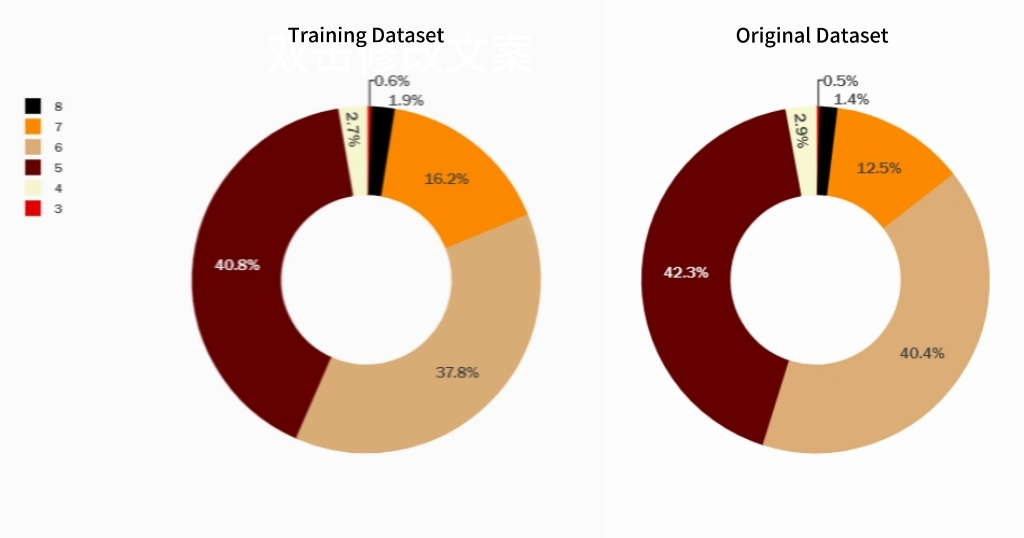
\includegraphics[width=0.9\linewidth]{TargetVariableAnalysis2.png}
			\end{tikzfigure}
			\begin{tikzfigure}
				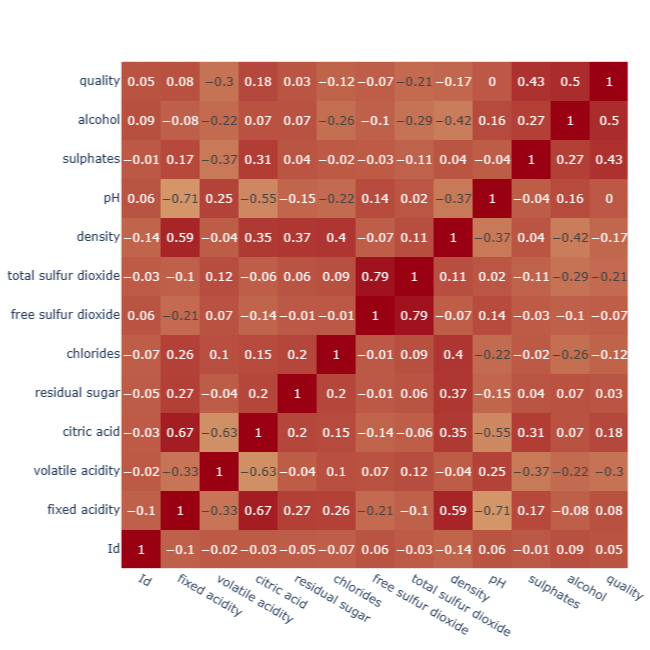
\includegraphics[width=0.9\linewidth]{CombinedTrainingDataset1.png}
			\end{tikzfigure}
		}
		
		
		
		\block{Experiment and analysis}{
			Subsequently, we quantified the number of samples for each quality level within the combined training dataset, revealing a class imbalance.Consequently, the Synthetic Minority Over-sampling Technique (SMOTE) was employed to oversample the dataset, resulting in the creation of a SMOTE-enhanced training set. The distribution of quality samples within this SMOTE training dataset was then meticulously documented.
			
			
		}
		%%%%%%%%%% -------------------------------------------------------------------- %%%%%%%%%%
		
		%%%%%%%%%% -------------------------------------------------------------------- %%%%%%%%%%
		\block[titlewidthscale=1, bodywidthscale=1]
		{Conclusion}
		{
			
			In scenarios where models are trained using both the combined training dataset and the SMOTE-enhanced training dataset, there is no significant difference in their performance on the validation set; however, training with the SMOTE-enhanced dataset enhances model performance on the training set. This suggests that the SMOTE method may assist in improving the model's fit to the training data, particularly in cases involving class imbalance in datasets.
			
		}
		%%%%%%%%%% -------------------------------------------------------------------- %%%%%%%%%%
		
		
	\end{columns}
	
	
	%%%%%%%%%% -------------------------------------------------------------------- %%%%%%%%%%
	\colorlet{notebgcolor}{blue!20}
	\colorlet{notefrcolor}{blue!20}
	\note[targetoffsetx=-13cm, targetoffsety=-8.5cm,rotate=0,angle=180,radius=8cm,width=.96\textwidth,innersep=.4cm]
	{
		\begin{minipage}{0.3\linewidth}
			\centering
			
\includegraphics[width=24cm]{./graphics/logos/tulip-wordmark.eps}
		\end{minipage}
		\begin{minipage}{0.7\linewidth}
			{ \centering
				The $11^{th}$ International Conference on Knowledge Science,
				Engineering and Management (KSEM 2018),
				17-19/08/2018, Changchun, China
			}
		\end{minipage}
	}
	%%%%%%%%%% -------------------------------------------------------------------- %%%%%%%%%%
	
	
\end{document}
